\Chapter{Minták generálása}

Tanító mintapontok előállítása

A megvalósító neurális hálózat betanítása felügyelt tanulás módszerrel történik. A minták alapján történő tanulás lényege, hogy az eljárás során a be és kimeneti mintapárokból igyekszünk megfelelő ismereteket kinyerni és ezzel a rendszer viselkedését módosítani. A hálózat feladata, hogy megtanulja a rendelkezésre álló mintapont párok által reprezentált bemenet-kimenet leképezést. Ehhez elő kell állítani a megfelelő adathalmazt.

Az adathalmaz előállítása elött definiálni kell a rajzolás dinamikáját. A vonal kirajzolás sorrendje mellet fontos a vonal vastagsága is. Az kézírás ugyan sokat változott, de az alapjai megmaradtak. A stroke-ok vastagsága az ecset gyorsaságától, az ecsetre ható nyomás nagyságától függ. A megfelelően rajzolt vonalakat nagyon fontosnak tartják a kínaiak, mivel a kultúrájukhoz tartozik. A kalligráfia elárulhatja az ember nemét, korát, személyességét és így tovább.

\begin{center}
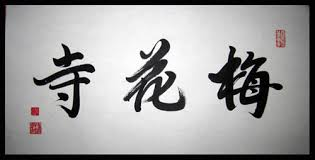
\includegraphics[scale=0.8]{calligraphy}
\end{center}

A következőkben részletezném a vonal vastagság változását a stroke-ok rajzolásának függvényébe. 

\begin{itemize}
\item A stroke-ok vége elvékonyul, ezt a valóságban az ecset hirtelen felemelésével érik el. (\textit{Van néhány kivétel: right fally} 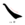
\includegraphics[scale=1.0]{right_fally}) 
\item Ha egy stroke végéből kezdődik egy másik stroke, akkor azok találkozásánál a vonalvastagság növekszik.
\item A horizontális vonalak közepe elvékonyul majd a végén újra vastagabb lesz. A vastagságot súlyokkal könnyedén lehet definiálni.

\begin{center}
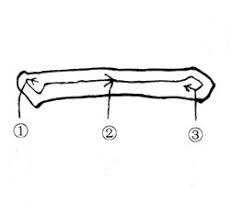
\includegraphics[scale=0.6]{horizontal_line}
\end{center}

\item A kampós vonalaknál (hooked stroke) a "kampó" hirtelen vékonyodással és irányváltoztatással jár. Az ecset hirtelen felemelésével érik el. Általában a kampó 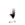
\includegraphics[scale=1.0]{hook} stroke része.
\item A további stroke-ok általában állandó vonal vastagsággal (ecset gyorsaság állandó). A kézzel írás és festés egyén függő.
\end{itemize}

A vastagság implementálásának módjai
\begin{itemize}
\item Súlyok 

\item Sebesség 

\item Szín átmenet 


\end{itemize}

Környezet
\begin{itemize}
\item Papír -> Képernyő
\item Ecset -> Ellipszis és azokat összekötő poligonok (OpenCV példa)
\item Karakter kombinációk (stroke sorrend) -> Lehet számozással, tömben deklarálva, mátrix térkép szerint stb..
\item Elrendezés, karakterek közötti távolság -> Viszony párokkal, láncolt lista (stroke párokkal).
\end{itemize}

\textit{Line break}\\\\

\begin{itemize}
\item Ecset dinamika
	\begin{itemize}
	\item \(P_1 = (x_1, y_1, d_{x_1}, d_{y_1}, s_1)\) \(P_2 = (x_2, y_2, d_{x_2}, d_{y_2}, s_2)\)
	\item Ecset szín (átmenetesség)
	\end{itemize}
\item Karakter kirajzolás
	\begin{itemize}
	\item Poligonos közelítés
	\item Procedurális rajzolás
	\item Pontonkénti színszámítás (fekete-szürke árnyalat-fehér)
	\item \textit{Görbék kirajzolása (Hermit)}
	\end{itemize}
\item Ideális karakter megjelenítés
\item Ideális karakter zajosítássa
	\begin{itemize}
	\item Különböző zajok
	\item Hálózat robosztussága
	\end{itemize}
\end{itemize}

\begin{comment}{Dolgozok a Hermit-es részen.}
\end{comment}

\begin{comment}{Ezek így vázlatnak jók, viszont az egyes pontokból legalább külön-külön szakaszoknak kellene majd lenni!}
\end{comment}
